%\begin{figure}
%\centering
%\subfloat[]{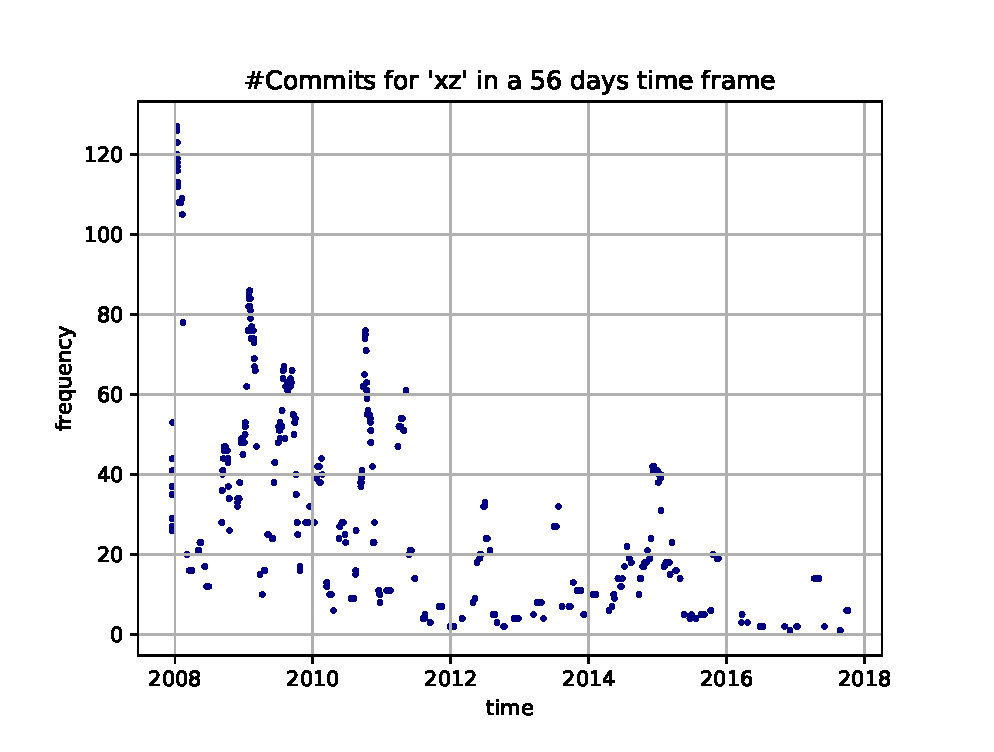
\includegraphics[width=0.4\textwidth]{images/activity_xz.eps}} 
%\subfloat[]{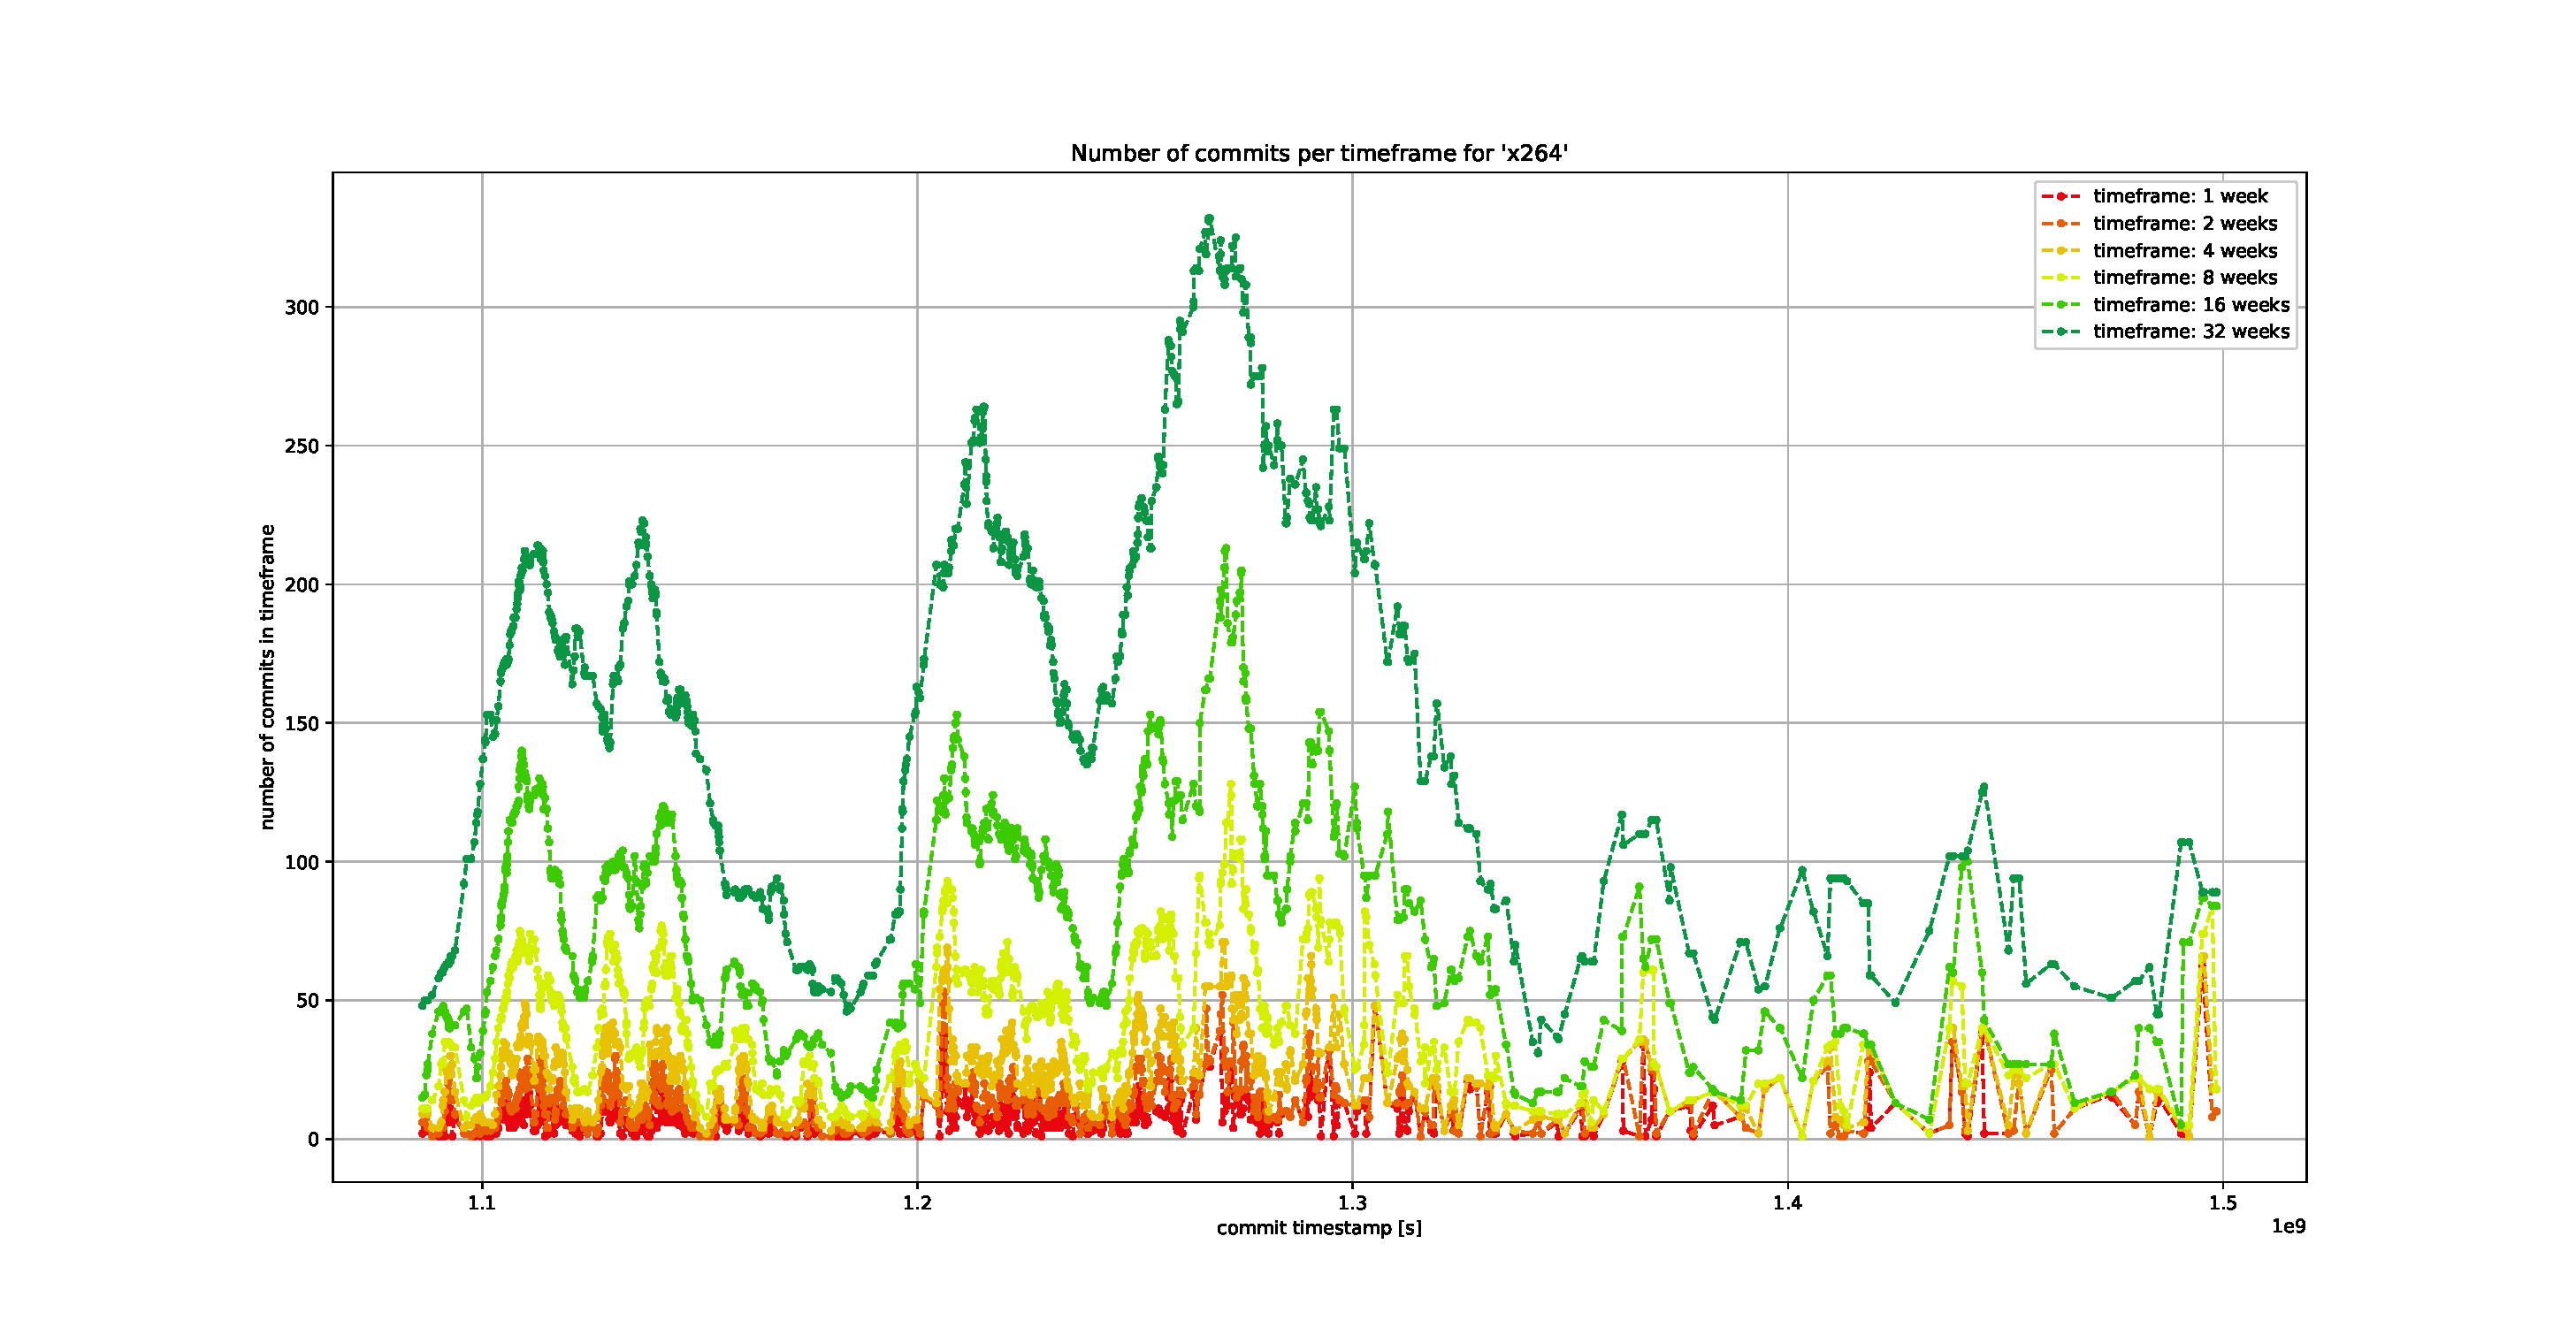
\includegraphics[width=0.4\textwidth]{images/activity_x264.eps}}
%\caption{Potential for 0.5 V bias.} 
%\label{fig:EcUND} 
%\end{figure} 

The assessment of performance evolution for a software system entails the
assessment of changes in performance measures over multiple versions of a
software system. To comprehend its version history, there exists a variety of
resources that can be employed, ranging from logs of a version control system
(VCS), such as Git, SVN, or CVS, over more elaborate documentations, such as
bug reports, to domain- or developer knowledge regarding the evolution of the
software system, such as requirement artifacts or mailing history. While VCS
logs usually record all fine-grained and iterative changes, bug reports or
release notes sketch larger chunks of the software evolution. Moreover, all
different resources focus on certain aspects of the software system’s
evolution, so that, for instance, VCS logs enable a developer-centered
perspective, whereas bug reports or release notes represent a more
user-centered perspective. That is, the assessment of performance for multiple
revisions of a software system always is placed in a certain context, such as
performance evolution of end-user versions when assessing releases only.

To understand how performance of a software system evolves in practice, it is
necessary to learn from which perspective we can observe and reenact
performance evolution for two reasons. \emph{First}, performance quality is a
concern which is omnipresent throughout development and usage of a software system.
Ideally, performance is avoided or handled during development, yet, not least
due to insufficient assessment (cf. Section 2), performance defects heavily
impact end-user satisfaction. \emph{Second}, we aim not to only understand
performance evolution, but to design tools leveraging this knowledge, for instance, to
predict performance for future changes, or to highlight performance-critical
code sections. For this purpose, efficient strategies to assess multiple
versions are inevitable.

Research so far has addressed the assessment of a software system’s revision
history under the umbrella of repository mining, for instance, to localize bugs
(Moin \& Khansari, 2010) or to XY. Nonetheless, so far there exists little to no
research addressing the question what perspective of version-related resources
as well as the choice of versions might reveal about performance evolution. The
task of selecting resources and a sample set of versions to analyze can be
conceived as a sampling strategy, where the objective is to cover interesting
entities (performance changes, in our case) while limiting the sample size to
keep the effort necessary reasonable. In this section, we develop and discuss
three sampling strategies to select versions from the overall version history.
These sampling strategies are subsequently applied to a selection of
configurable software systems and evaluated in the remainder of this thesis.


\begin{figure}
\def\tabularxcolumn#1{m{#1}}
\begin{tabularx}{\linewidth}{@{}cXX@{}}
\begin{tabular}{c}
\subfloat[Activity Graph for \texttt{GNU XZ}, generated from 399 versions
between March 24, 2017, and August 14, 2017. The earliest release version is
\texttt{5.1.1alpha}, the latest is \texttt{5.3.0alpha}.]
{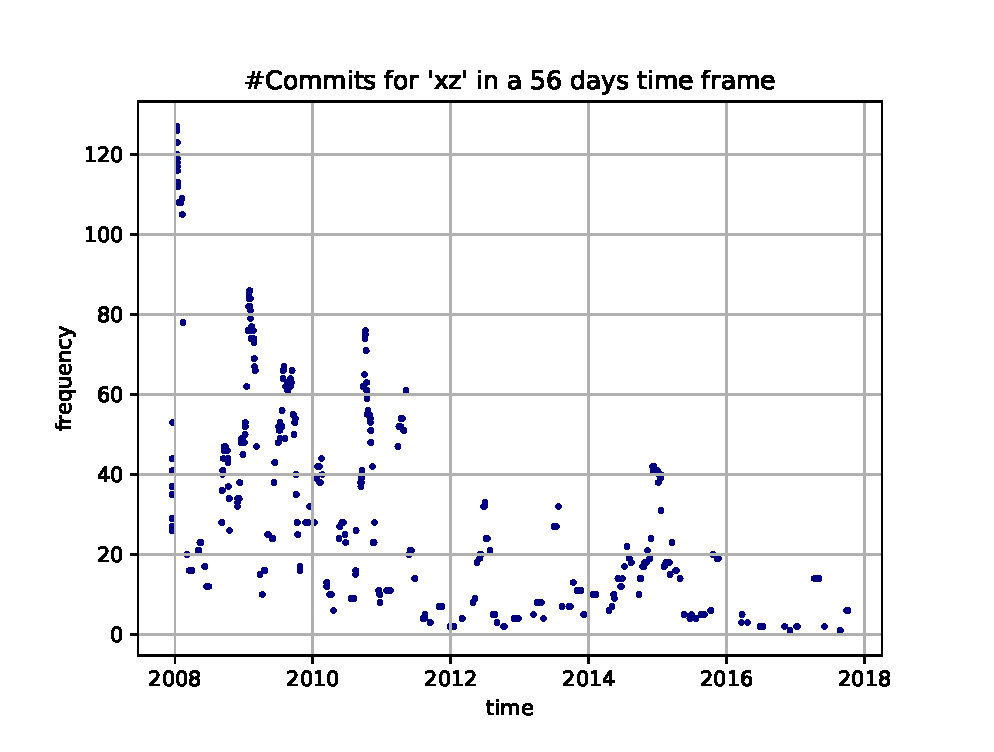
\includegraphics[width=0.99\textwidth]{images/activity_xz.eps}}
\\
\subfloat[Activity Graph for \texttt{x264}, generated from 2851 versions
between June 3, 2004, and June 26, 2017. The earliest release version is
\texttt{BUILD 1} from, the latest is \texttt{BUILD 149} from
X.]{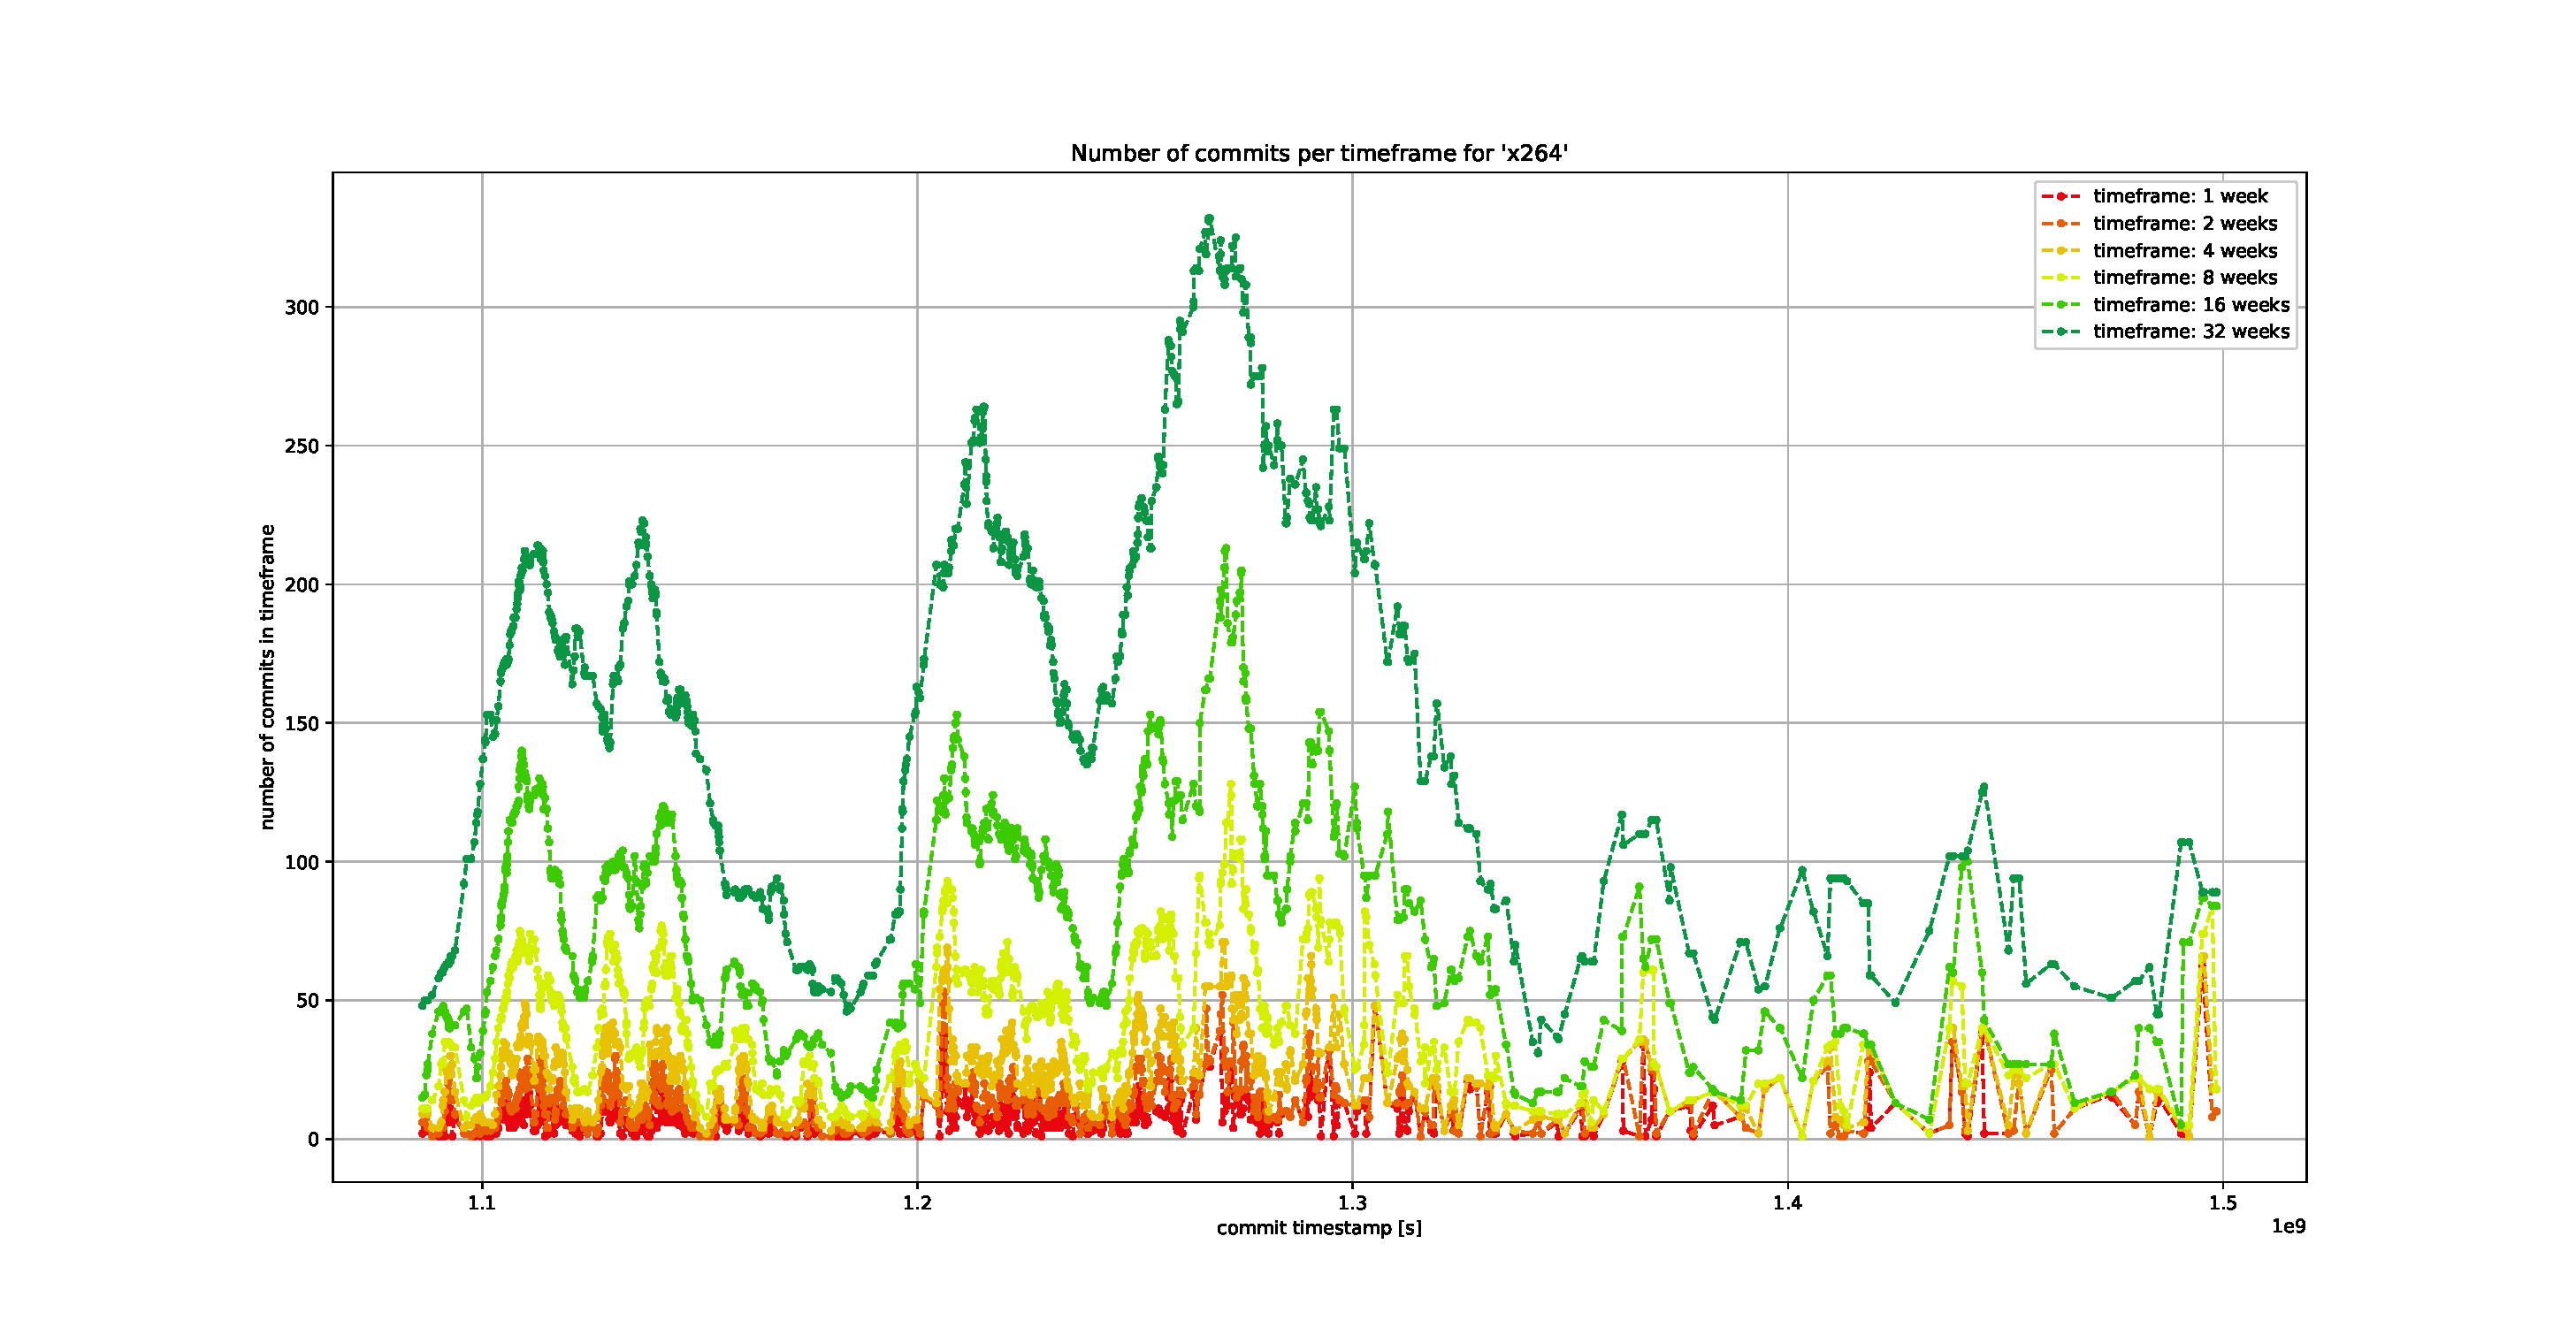
\includegraphics[width=0.99\textwidth]{images/activity_x264.eps}}\\
\end{tabular}
\end{tabularx}
\caption{Commit activity for two sample systems, the compression
utility \texttt{GNU XZ} and the video encoder \texttt{x264}. For each version,
the activity is measured as the number of commits that were pushed within a
certain timeframe after or before the actual commit. The timeframes range from
one week to 32 weeks, as shown in the legendary.}
\label{fig:ActivityGraphs}
\end{figure}


\section{Sampling Strategy Approaches}
\begin{itemize}
  \item End-User-Centric or Release Sampling
  \item Segmentation Sampling
  \item Defect-Centric sampling
  \item Hot-Spot sampling
\end{itemize}
\section{Sampling Strategy Classification}
